\chapter{Knowledge gain with multiple episodes}
\begin{quotation}
\noindent ``\emph{quote}''
\begin{flushright}\textbf{author}\end{flushright}
\end{quotation}

We will first and foremost analyse how a reinforcement learning agent 
performs when it is confronted to playing a single episode of one of the 
CartPole problems. We will train the agent on a distribution of 20 permutations
(shown on Table~\ref{tab:20perms}), at first without inverting the agent's
action.\\

\begin{table}
	\centering
	\caption{State permutations used for training and testing}
	\label{tab:20perms}
	\subfloat[Training distribution]{
		\bgroup
		\def\arraystretch{1.5}
		\begin{tabular}{c|c|c}
			[0, 1, 2, 3] & [1, 0, 2, 3] & [2, 0, 1, 3] \\
			\hline
			[0, 1, 3, 2] & [1, 0, 3, 2] & [2, 0, 3, 1] \\
			\hline
			[0, 2, 1, 3] & [1, 2, 0, 3] & [2, 1, 0, 3] \\
			\hline
			[0, 2, 3, 1] & [1, 2, 3, 0] & [3, 0, 1, 2] \\
			\hline
			[0, 3, 1, 2] & [1, 3, 0, 2] & [3, 0, 2, 1] \\
			\hline
			[0, 3, 2, 1] & [1, 3, 2, 0] & [3, 1, 0, 2] 
		\end{tabular}
		\egroup
	}
	\subfloat[Testing distribution]{
		\quad\quad
		\bgroup
		\def\arraystretch{1.5}
		\begin{tabular}{c}
			[2, 1, 3, 0] \\
			\hline
			[2, 3, 0, 1] \\
			\hline
			[2, 3, 1, 0] \\
			\hline
			[3, 1, 2, 0] \\
			\hline
			[3, 2, 0, 1] \\
			\hline
			[3, 2, 1, 0]
		\end{tabular}
		\egroup
		\quad\quad
	}
\end{table}

As a control experiment, we first need to check whether the agent can learn
to discover which permutation of the state has been selected and to keep the
pole balanced within one single episode. Surprisingly, as shown in 
Figure~\ref{fig:20perms1ep_training}, the agent quickly manages to reach
a very good performance level, only failing a small percentage of the time.\\

When the agent is trained on trials of 2 episodes, we expect that its
performance will improve (however good it already is). Looking at the graph 
of Figure~\ref{fig:20perms2ep_training}, we can only deduce two things : 
\begin{enumerate}
	\item the performance of the first episode of every trial drops 
		significantly compared to trials of one episode;
	\item the performance of the second episode of every trial matches
		closely the performance of single-episode trials.
\end{enumerate}
The second of these considerations will be addressed in
chapter~\ref{chap:reward_structure}. Let us analyse the first one in more detail
as the average reward graph doesn't give us enough insight in the final
reward distributions.\\

\begin{figure}
	\centering
	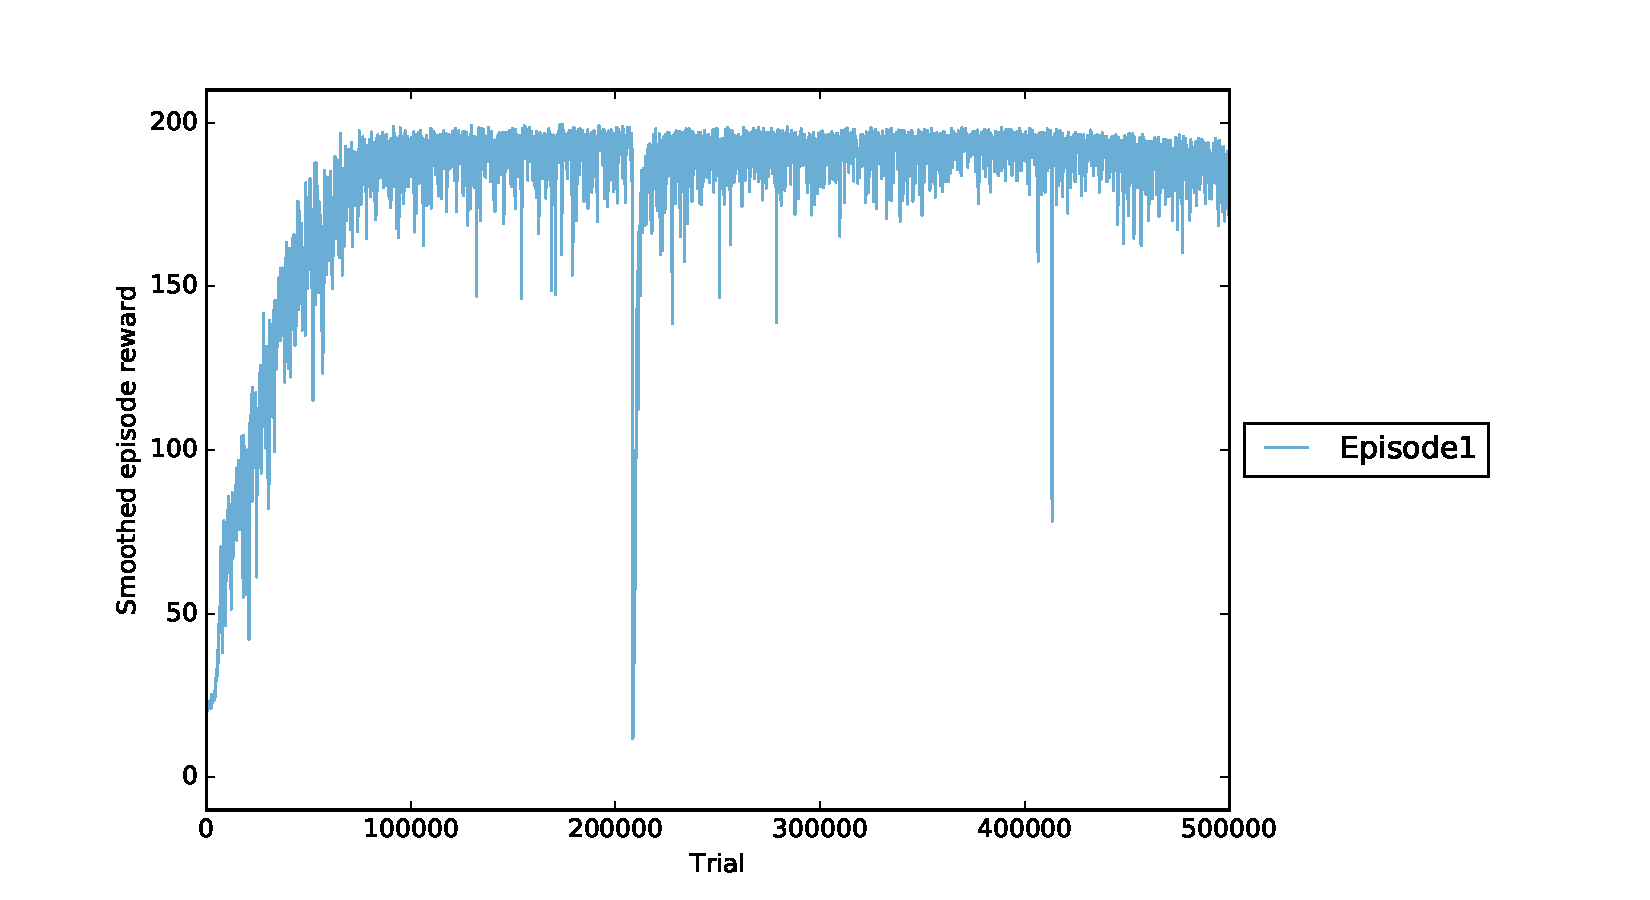
\includegraphics[width=0.9\linewidth]{fig/20perms1ep_training.pdf}
	\caption{Training of an agent on trials of 1 episode. The curve
	shows a moving average over 200 trials.}
	\label{fig:20perms1ep_training}
\end{figure}


\begin{figure}
	\centering
	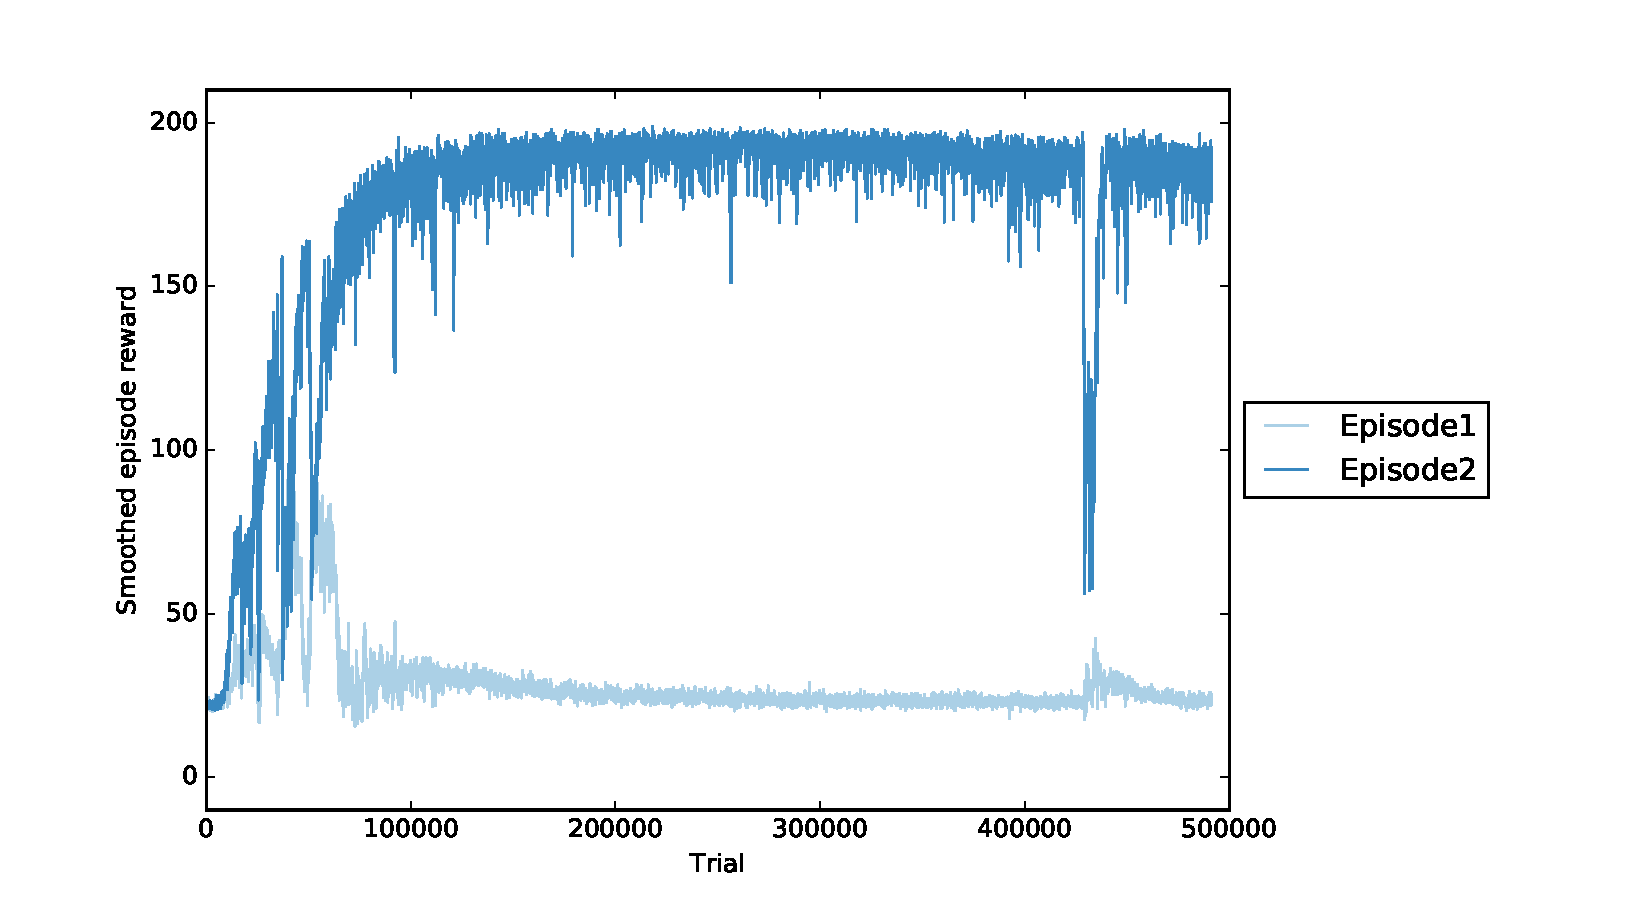
\includegraphics[width=0.9\linewidth]{fig/20perms2ep_training.pdf}
	\caption{Training of an agent on trials of 2 episodes}
	\label{fig:20perms2ep_training}
\end{figure}

Let us compare the final reward distribution for the only episode of 
single-episode trials and for the second episode of dual-episode trials.
For now, we are not interested in the reward distribution of the first episode
in dual-episode trials as we want to see whether or not the agent managed to
gain knowledge during that first episode (potentially hurting its first episode
reward) to improve its performance for the second episode.\\

To compare the two settings, we fix the agent's learnable parameters and make
it play 180 trials (resetting its hidden state before every trial). Every 
CartPole problem in the distribution is played the same amount of times. \\

Figure~\ref{fig:20perms_distrib} shows both a histogram and a boxplot describing
the final reward distributions in the single and dual episode situations. 
Although the difference is slight, and seeing that the number
of successes (a final reward of 195 or more, corresponding to the uppermost
bar) is almost exactly the same, there is definitely a difference in when the
failures occur. For the single episode setting, all failures are distributed
in a relatively uniform way spanning from 50 to 195; whereas they cluster 
slightly above 150 in the dual episode setting. The boxplots clearly show
a more compact distribution (and so a generally higher reward) in the dual
episode setting.\\

The agent seems to learn from the first episode to improve its performance in
the second. This is even clearer when we run the same experiment on unseen
permutations. As shown on Figure~\ref{fig:20perms_unseen_distrib}, where the
agent played every permutation of the test set for 30 trials, playing 180
trials in total to allow for comparison to the previous experiment, the agent
playing single-episode trials fails more often with a reward around 50. The
dual-episode setting shows again a capability to learn from the first episode
to improve performance in the second.\\

\begin{figure}
	\centering
	\subfloat[][Trials of 1 episode]{
		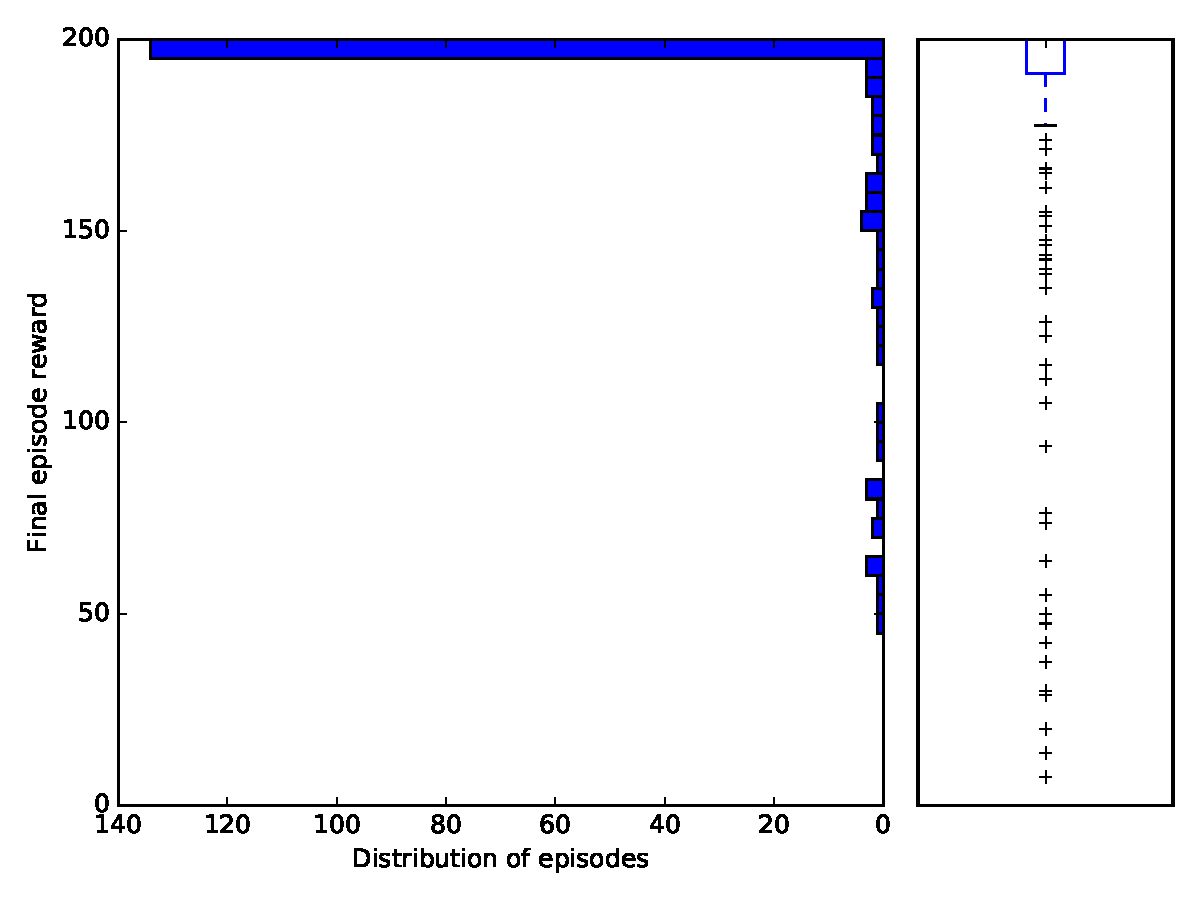
\includegraphics[width=0.49\linewidth]{fig/20perms_distrib_1ep.pdf}}
	\subfloat[][Trials of 2 episodes]{
		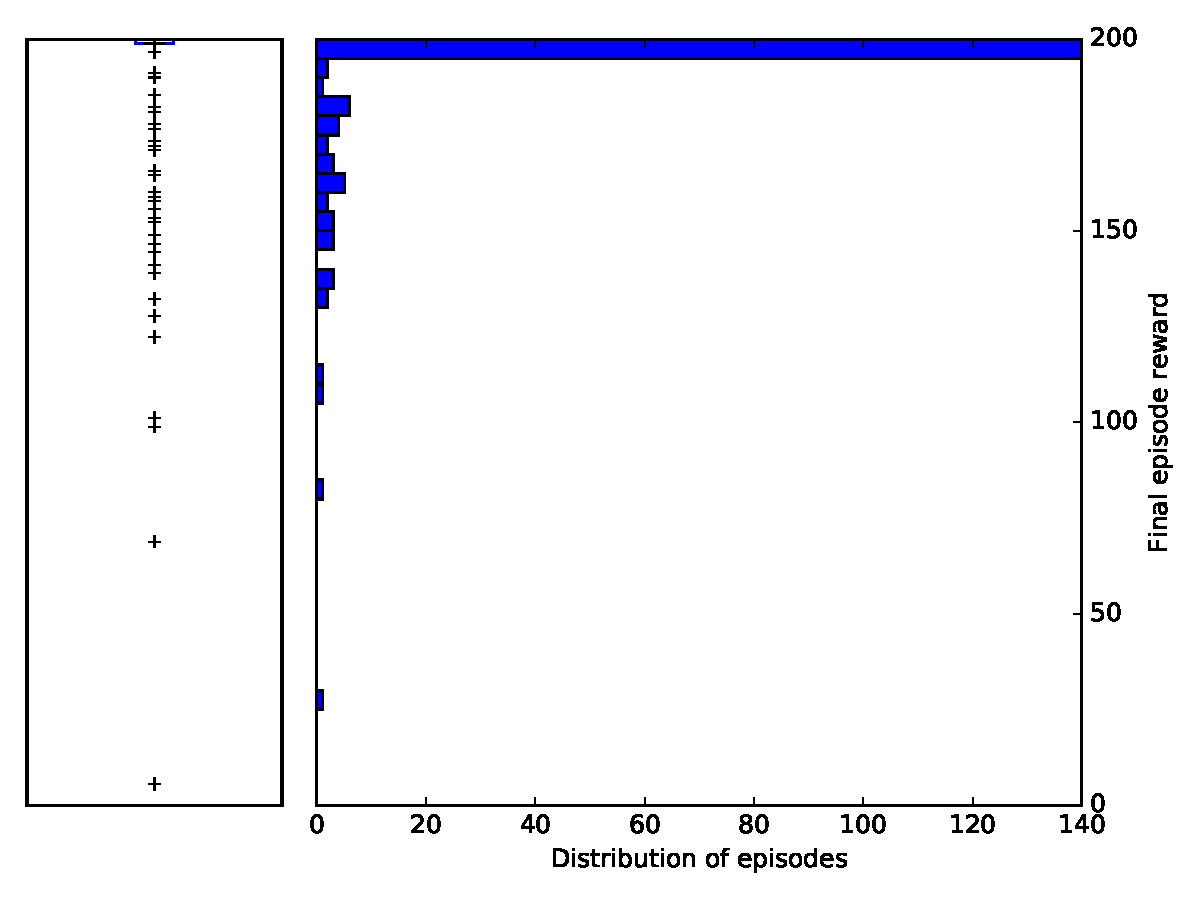
\includegraphics[width=0.49\linewidth]{fig/20perms_distrib_2ep.pdf}}
	\caption{}
	\label{fig:20perms_distrib}
\end{figure}
\todo{captions}

\begin{figure}
	\centering
	\subfloat[][Trials of 1 episode]{
		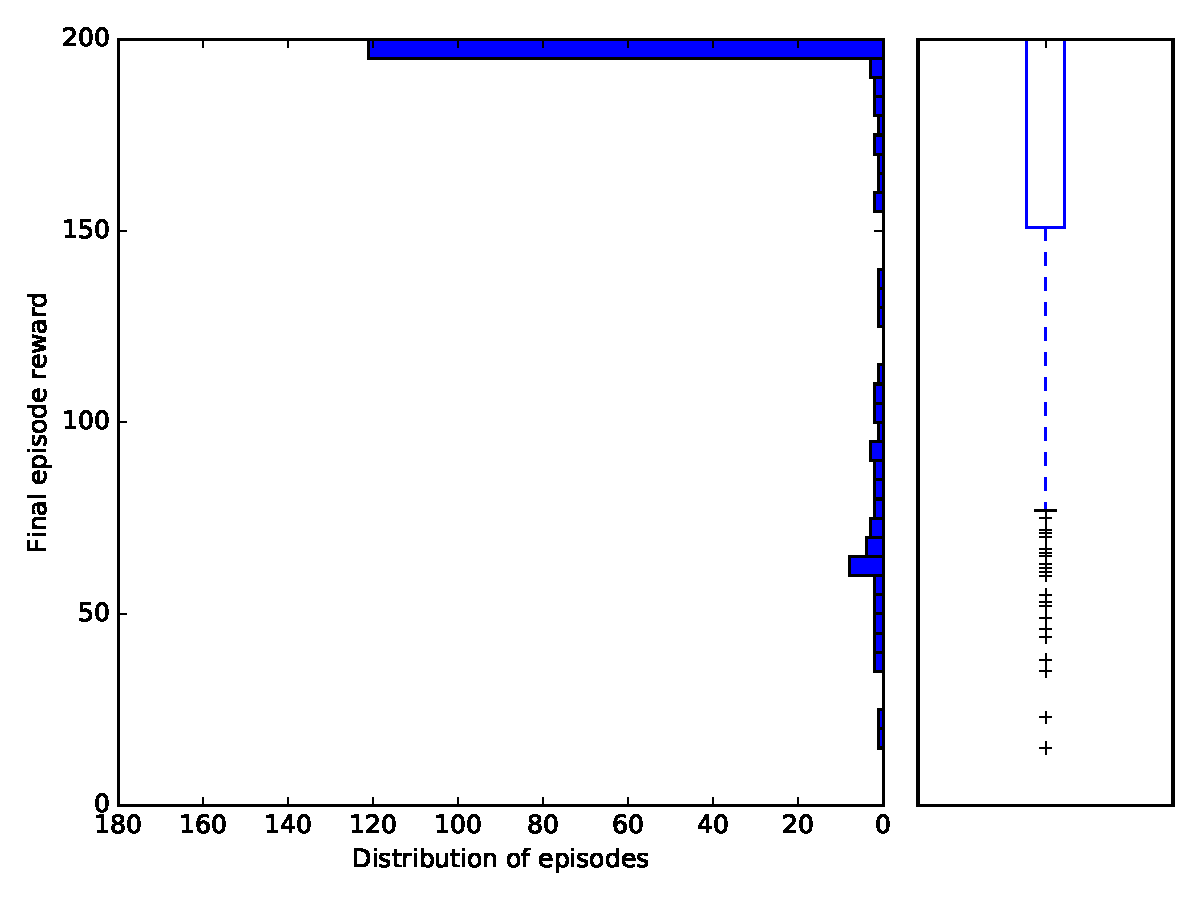
\includegraphics[width=0.49\linewidth]{fig/20perms_unseen_distrib_1ep.pdf}}
	\subfloat[][Trials of 2 episodes]{
		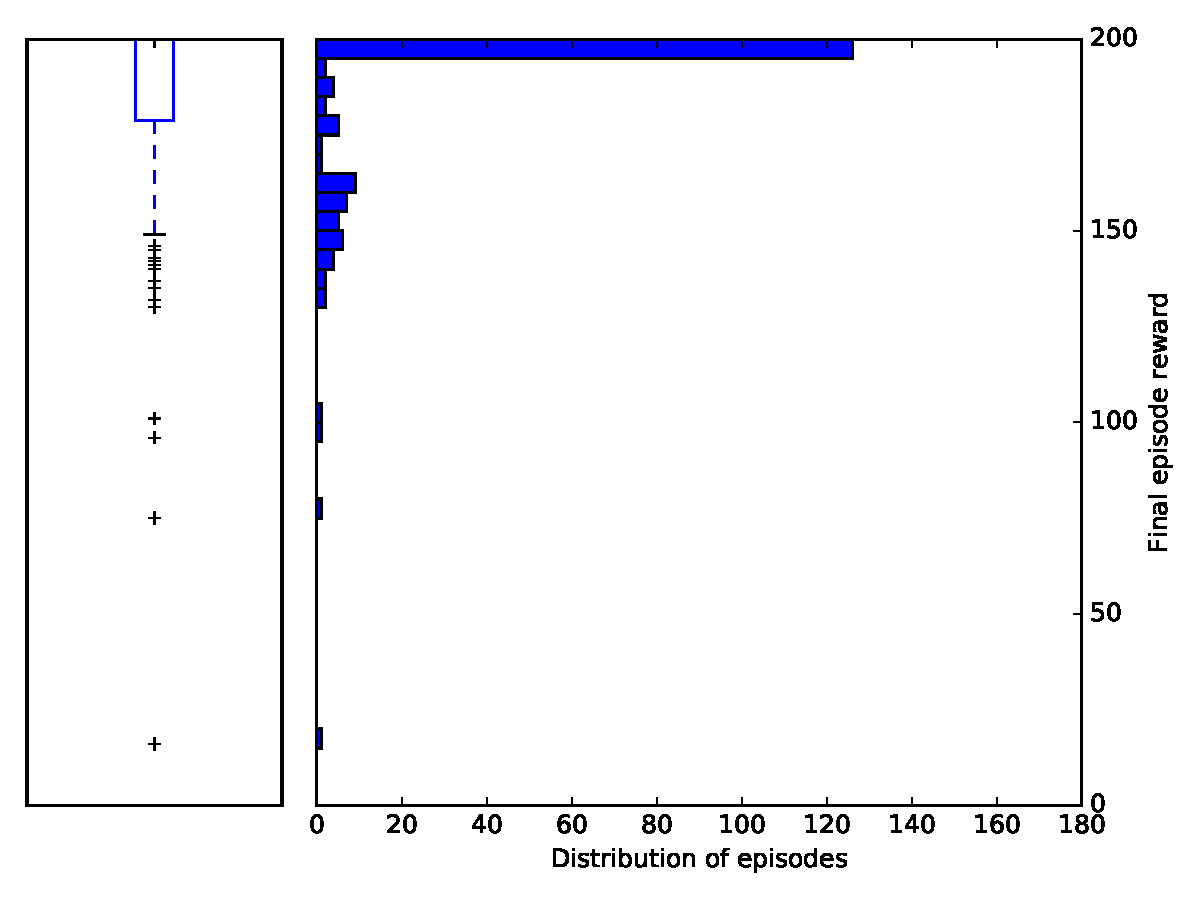
\includegraphics[width=0.49\linewidth]{fig/20perms_unseen_distrib_2ep.pdf}}
	\caption{}
	\label{fig:20perms_unseen_distrib}
\end{figure}

Even more impressingly, if we add the inversion of the left and right actions
with a probability of 0.5 at the start of every trial, this effect is
tremendously magnified. For seen permutations
(Figure~\ref{fig:20permsLR_distrib}), there are about 40 more successes (out of
180) when playing two episodes than when playing only one; for unseen
permutations, this number climbs to about 70 out of 180. The single-episode
agent succeeds shy of 100 trials out of 180 where the dual-episode agent
comes close to 170 out of 180.\\

\begin{figure}
	\centering
	\subfloat[][Trials of 1 episode]{
		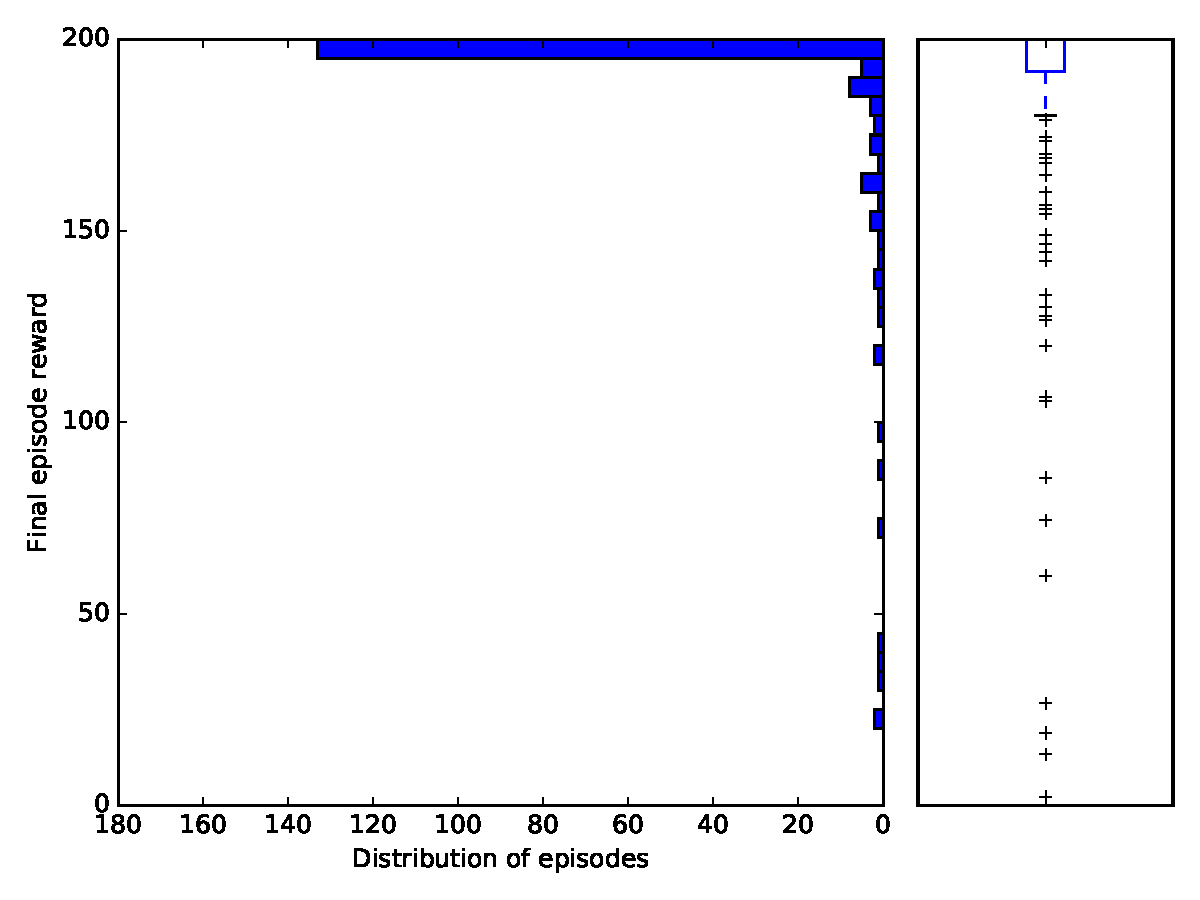
\includegraphics[width=0.49\linewidth]{fig/20permsLR_distrib_1ep.pdf}}
	\subfloat[][Trials of 2 episodes]{
		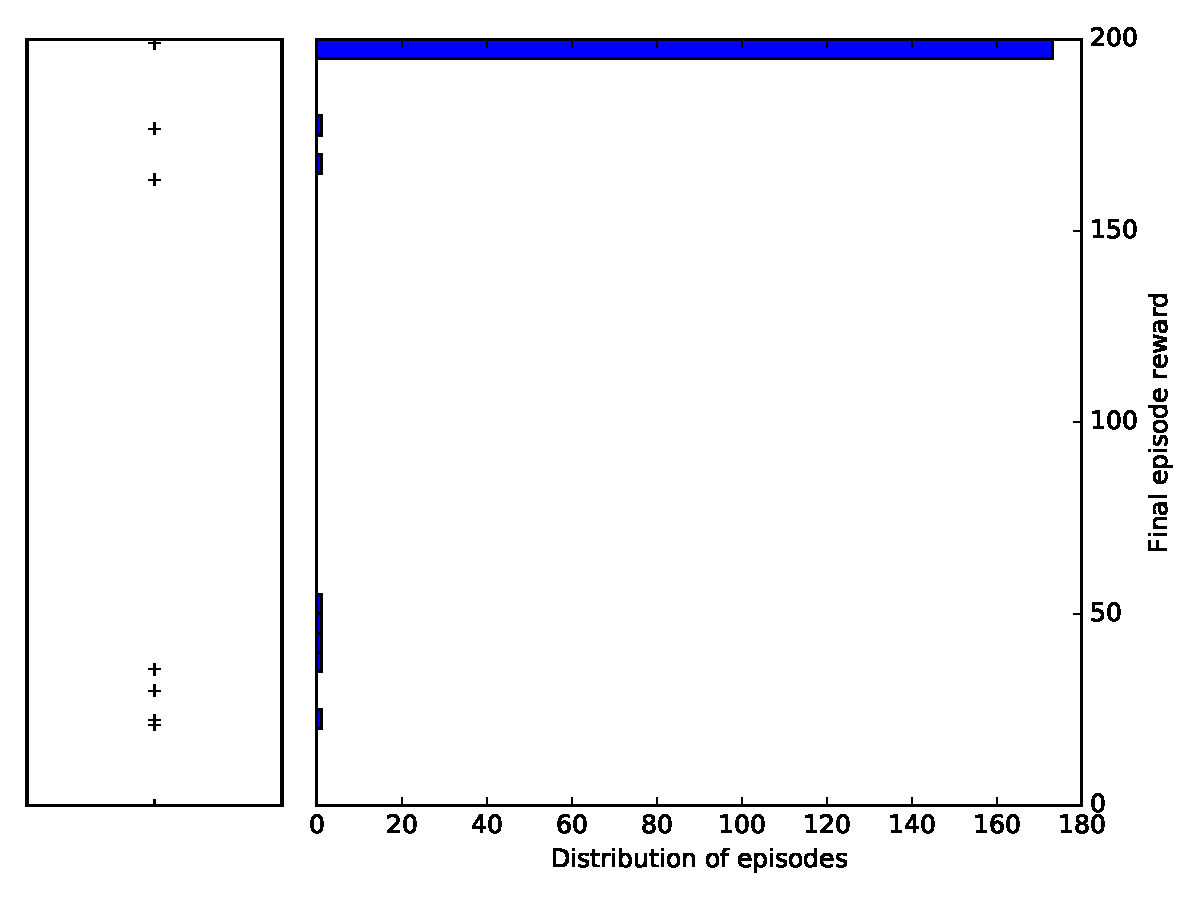
\includegraphics[width=0.49\linewidth]{fig/20permsLR_distrib_2ep.pdf}}
	\caption{}
	\label{fig:20permsLR_distrib}
\end{figure}

\begin{figure}
	\centering
	\subfloat[][Trials of 1 episode]{
		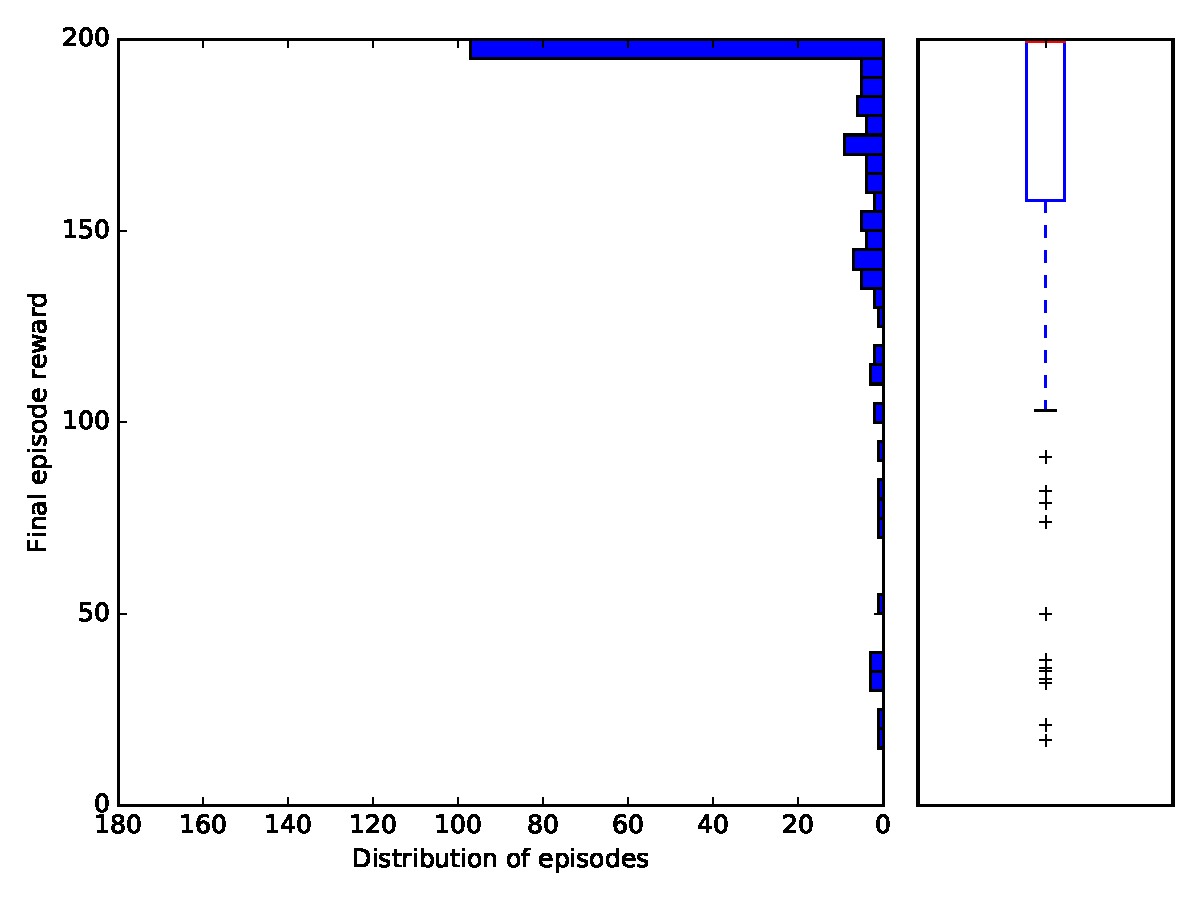
\includegraphics[width=0.49\linewidth]{fig/20permsLR_unseen_distrib_1ep.pdf}}
	\subfloat[][Trials of 2 episodes]{
		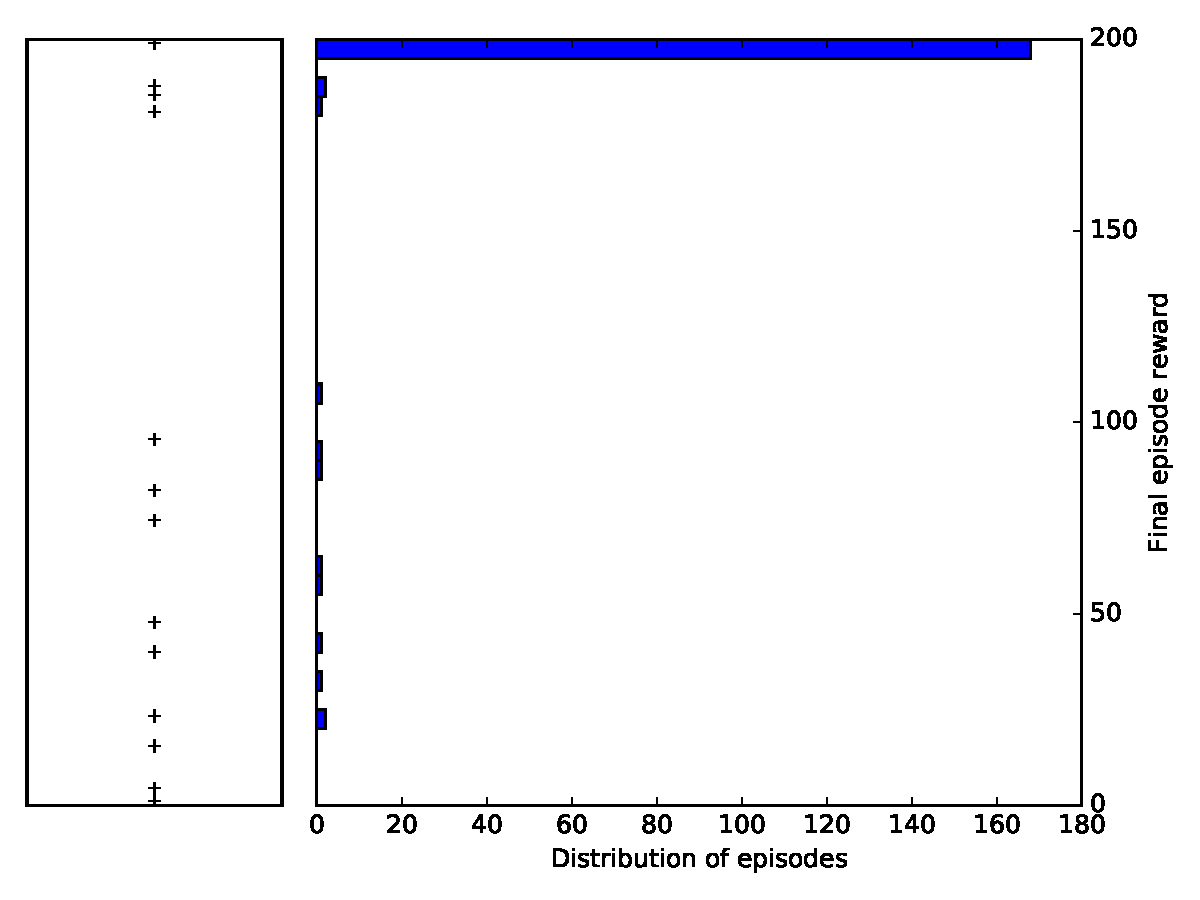
\includegraphics[width=0.49\linewidth]{fig/20permsLR_unseen_distrib_2ep.pdf}}
	\caption{}
	\label{fig:20permsLR_unseen_distrib}
\end{figure}

There are several surprises in these results. The first one is that a single
episode appears to be enough for an agent to discover how the observation has
been permutated in time to take action so that the pole stays balanced (at least
for a majority of trials), but playing a second episode improves the performance
of the agent.\\

The second one seems to be that in the setting of dual-episode trials, the
harder the problem is, the higher the number of successes will be. Indeed,
the performance of agents playing problems with inverted actions is 
significantly higher than the performance of agents playing problems without.





